\documentclass[10pt,a4paper]{article}

\usepackage[T1]{fontenc}
\usepackage[utf8]{inputenc}
\usepackage[margin=18mm]{geometry}
\usepackage{booktabs}
\usepackage{graphicx}
\usepackage{xcolor}
\usepackage{hyperref}
\usepackage{enumitem}
\usepackage{caption}

\definecolor{accent}{HTML}{1D4ED8}
\definecolor{muted}{HTML}{475569}
\hypersetup{
  colorlinks=true,
  linkcolor=accent,
  urlcolor=accent,
  pdfauthor={UWB Module project},
  pdftitle={Passive DS-TWR Known-Geometry Calibration}
}
\setlist{nosep,leftmargin=5mm}
\captionsetup{font=small,labelfont=bf}
\setlength{\parindent}{0pt}
\setlength{\parskip}{5pt}

\newcommand{\cm}{\,cm}
\newcommand{\mm}{\,mm}

\title{\vspace{-13mm}\textbf{Passive DS-TWR Known-Geometry Calibration}\\
\large Static receive-only tag validation}
\author{UWB Module project}
\date{27 July 2026}

\begin{document}
\maketitle
\vspace{-5mm}

\begin{abstract}
This report validates the project-specific Passive DS-TWR protocol after
restoring a surveyed four-anchor geometry. Hardware-bias calibration reduces
the live position-bias magnitude from \(3.51\cm\) to \(0.96\cm\). The embedded
solver improves from \(4.12\cm\) to \(3.33\cm\) 2-D RMSE. Re-solving the same
calibrated observations with the surveyed geometry reaches
\textbf{\(1.89\cm\) RMSE and \(3.11\cm\) P95 at \(49.17\) complete frames/s}.
The remaining live accuracy penalty is therefore dominated by autonomous
anchor-geometry reconstruction rather than by the passive observation
equation.
\end{abstract}

\section{Experimental setup}

Four anchors formed a surveyed \(3.000\) m square and tag 1 was placed at its
center:

\begin{center}
\begin{tabular}{@{}cc@{\hspace{14mm}}cc@{}}
\toprule
Node & Coordinate [m] & Node & Coordinate [m] \\
\midrule
A2 & \((0.000,\,0.000)\) & A3 & \((0.000,\,3.000)\) \\
A4 & \((3.000,\,0.000)\) & A5 & \((3.000,\,3.000)\) \\
Tag 1 & \((1.500,\,1.500)\) & Placement tolerance & approximately \(\pm2\mm\) \\
\bottomrule
\end{tabular}
\end{center}

Both independent captures lasted 120 s and used Robust Rotating scheduling,
5 ms slots, a 1 ms frame gap, 1000 us RESP and FINAL delays, and UWB channel 5.
The first capture used raw observations and raw piggybacked DS ranges. The
second capture used the calibration derived from the first capture.

\section{Position results}

\begin{center}
\small
\begin{tabular}{@{}lrrrrr@{}}
\toprule
Processing path & Positions & Rate [Hz] & Bias X/Y [cm] & RMSE [cm] & P95 [cm] \\
\midrule
Uncalibrated, autonomous geometry
  & 3,362 & 28.00 & \(+3.24/-1.35\) & 4.12 & 6.09 \\
Calibrated, autonomous geometry
  & 3,512 & 29.26 & \(-0.66/-0.70\) & 3.33 & 5.66 \\
Calibrated, surveyed geometry
  & 5,901 & 49.17 & \(-0.30/-0.27\) & \textbf{1.89} & \textbf{3.11} \\
\bottomrule
\end{tabular}
\end{center}

Calibration improves the live embedded RMSE by \(19.2\%\) and reduces the
systematic position-bias magnitude by \(72.7\%\). The HTTP snapshot collector
keeps only the newest embedded position, so its 28--29 samples/s is a capture
limit. Offline reconstruction of one solution per complete three-slot star
shows the actual \(49.2\) frames/s position cadence.

\begin{figure}[ht]
\centering
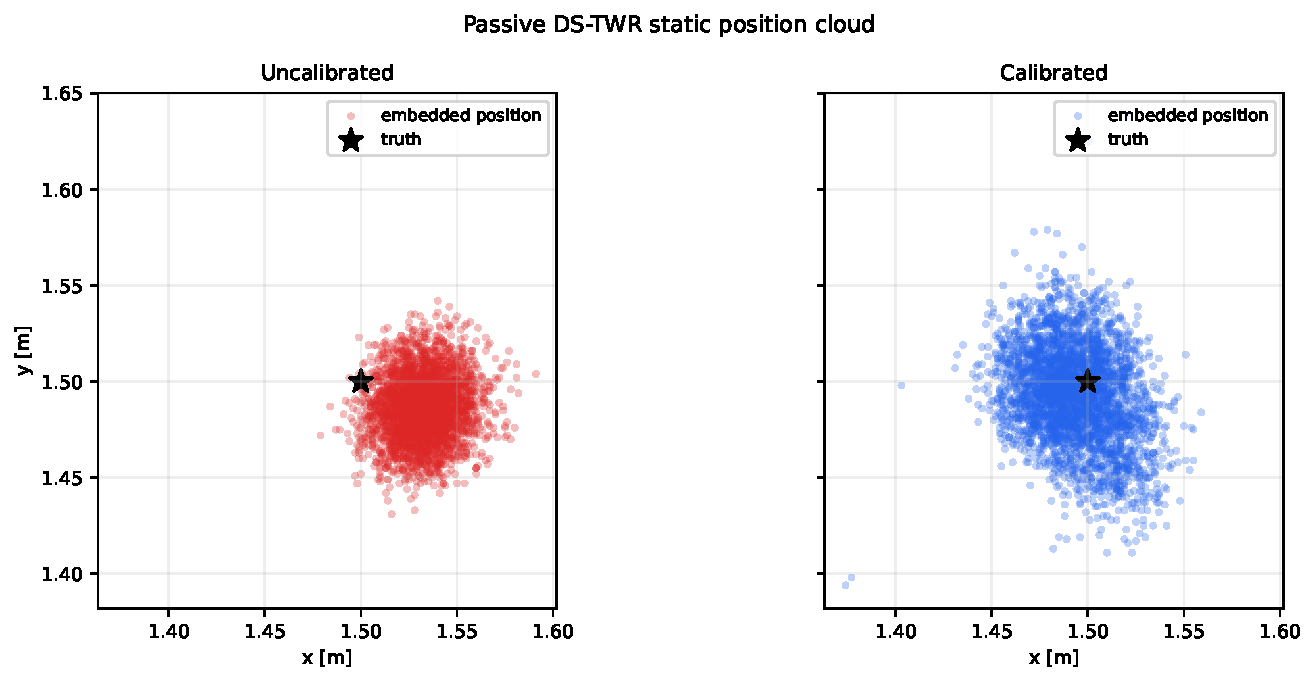
\includegraphics[width=\textwidth]{figures/position_scatter.pdf}
\caption{Embedded position clouds before and after calibration. The black star
is the surveyed tag position.}
\end{figure}

\begin{figure}[ht]
\centering
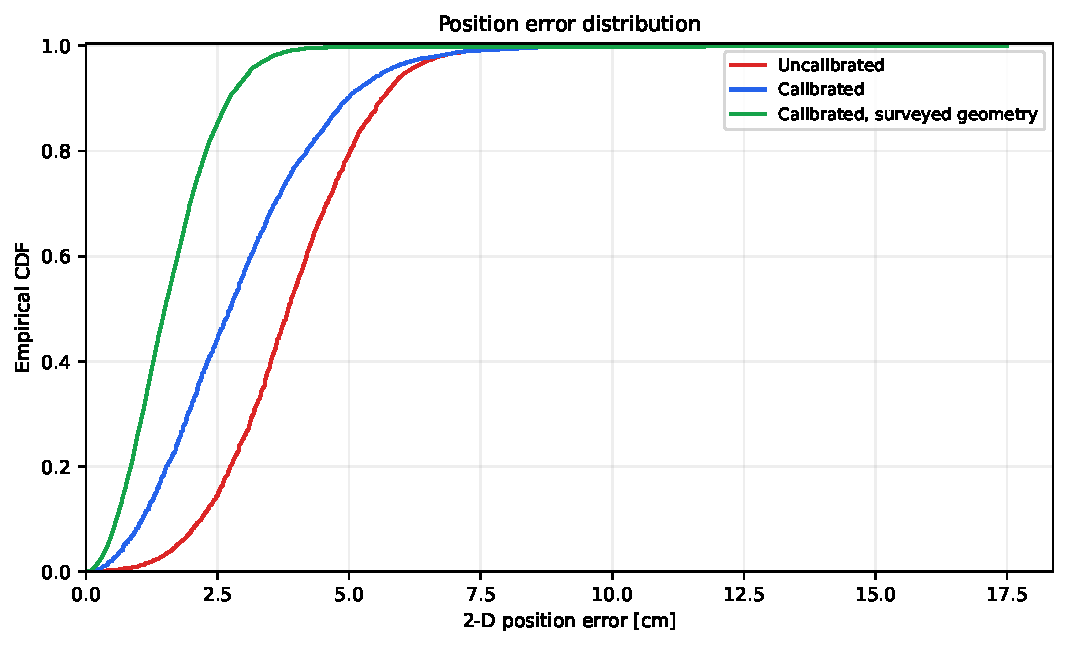
\includegraphics[width=0.86\textwidth]{figures/position_error_cdf.pdf}
\caption{Empirical 2-D error distributions. Replacing only the autonomous
geometry with surveyed coordinates exposes the quality of the calibrated
passive observations.}
\end{figure}

\clearpage
\section{Calibration model}

The scalable directed-observation model is
\[
  e_{I\rightarrow R}=b_R-b_I ,
\]
where \(b_I\) and \(b_R\) are per-anchor biases. A2 fixes the arbitrary common
offset. The first half of the uncalibrated observation capture produced:

\begin{center}
\begin{tabular}{@{}cr@{\hspace{13mm}}cr@{}}
\toprule
Anchor & Observation bias & Anchor & Observation bias \\
\midrule
A2 & \(0\mm\)   & A3 & \(+34\mm\) \\
A4 & \(-16\mm\) & A5 & \(-55\mm\) \\
\bottomrule
\end{tabular}
\end{center}

This uses only \(N-1\) independent values for \(N\) anchors while reproducing
the corrections for all 12 directed paths. The piggybacked DS ranges use one
additional correction per unordered anchor pair:

\begin{center}
\begin{tabular}{@{}cr@{\hspace{9mm}}cr@{\hspace{9mm}}cr@{}}
\toprule
Pair & Bias & Pair & Bias & Pair & Bias \\
\midrule
A2--A3 & \(+71\mm\) & A2--A4 & \(+56\mm\) & A2--A5 & \(-49\mm\) \\
A3--A4 & \(+67\mm\) & A3--A5 & \(+66\mm\) & A4--A5 & \(-29\mm\) \\
\bottomrule
\end{tabular}
\end{center}

\begin{figure}[ht]
\centering
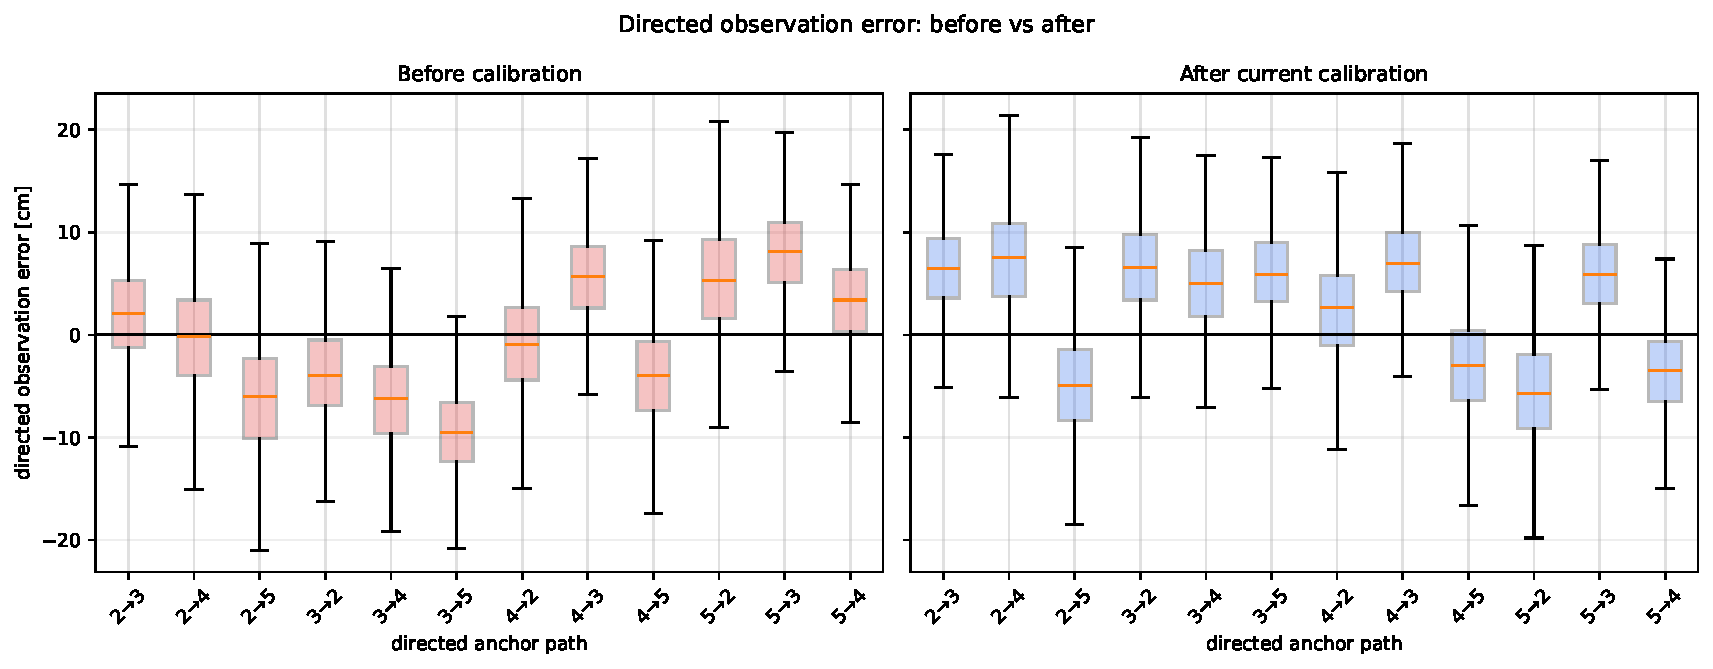
\includegraphics[width=0.82\textwidth]{figures/directed_observation_bias.pdf}
\caption{Uncalibrated error on each directed path. Opposite signs are
consistent with a compact per-anchor bias model.}
\end{figure}

\begin{figure}[ht]
\centering
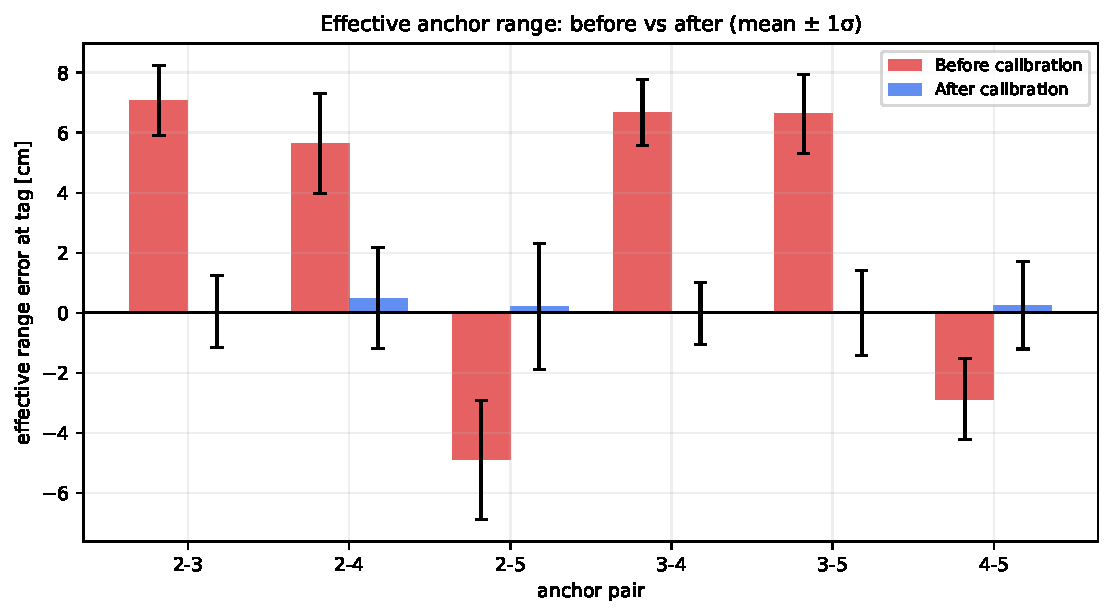
\includegraphics[width=0.72\textwidth]{figures/anchor_pair_range_bias.pdf}
\caption{Mean anchor-pair DS range error with one standard deviation.}
\end{figure}

\clearpage
\section{Protocol health and interpretation}

During the calibrated capture, anchor radio success ranged from \(97.37\%\) to
\(98.49\%\). The embedded calibrated distribution contains five estimates
above \(10\cm\) (\(0.142\%\)), including two above \(15\cm\). They are short
transients and remain included in every reported statistic and plot.

The uncorrected pair distances still fit a planar geometry with
\(1.99\cm\) range-residual RMS, but the resulting anchor coordinates are
displaced by several centimeters. Consequently:

\begin{itemize}
  \item CFO correction of the responder reply interval is working;
  \item passive directed observations benefit from the per-anchor bias model;
  \item piggybacked DS ranges benefit from per-pair corrections;
  \item autonomous geometry is now the largest remaining live accuracy
        penalty.
\end{itemize}

The next implementation step should robustly filter pair ranges before they
update geometry: a rolling median or Huber estimate, a physical-change gate,
and a slower geometry-update cadence. Validation should then cover several
static tag locations and a dynamic trajectory. A single center position
identifies the current bias, but cannot establish workspace-wide accuracy.

\section{Reproducibility}

The repository preserves both compressed JSONL captures, metadata, wireless
logs, SHA-256 manifests, CSV metrics, figures, and the deterministic analyzer:

\begin{verbatim}
python3 tools/uwb_passive_ds_known_geometry_analyze.py
\end{verbatim}

The complete machine-readable result is in
\path{analysis_summary.json}; detailed methodology is in \path{README.md}.

\vfill
\begin{center}
\color{muted}\small
Branch: \texttt{experiment/passive-ds-twr} \quad
Calibration firmware: \texttt{8db125e}
\end{center}

\end{document}
